\scanpage{63}

Notons d'ailleurs, pour le cas d'un entier $n$ ne satisfaisant pas \inserted{nécessairement} les conditions envisagées dans c):

\uline{Corollaire} \inserted{10}. Soit $n$ un entier. On a alors une suite exacte canonique
\diagram{\begin{tikzcd}[column sep=small]
(\unsure{11|10})\quad0\arrow[r]&{}_n\Gamma\arrow[r]&H^1(X,\mu_n)\arrow[r,"u_n"]&H^1(X_{\bar\eta},\mu_n)^I\arrow[r]&Q\deleted{{}_n}(n)\arrow[r]&0,
\end{tikzcd}}
où $Q_n=\operatorname{Coker}u_n$ s'insère dans une suite exacte canonique
\diagram{\begin{tikzcd}[column sep=small]
(12)\quad0\arrow[r]&\operatorname{Ker}w_n\arrow[r]&Q\deleted{{}_n}(n)\arrow[r]&\theta(n)\arrow[r]&0,
\end{tikzcd}}
avec
\[
(13)\qquad\theta(n)\unsure{\hookrightarrow|\subset}{}_n\operatorname{Ker}(\operatorname{Br}(K)\longrightarrow\operatorname{Br}(X_\eta))\hookrightarrow{}_{(n,d^t)}\operatorname{Br}(K),
\]
\margin{\figure{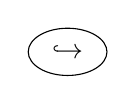
\begin{tikzpicture}\node at (0,0) {$\hookrightarrow$};\draw (0,0) ellipse (.5 and .3);\end{tikzpicture}}}
de sorte que l'on a $\theta(n)=0$ lorsque $n$ ou $d^t$ sont premiers à $p$ ou\deleted{\unsure{x}} que $k$ est parfait (donc $\operatorname{Br}(K)=0$). En tous cas, si $p^m$ est la plus grande puissance de $p$ divisant $d^t$ (qui est donc indépendant de choix de $n$), on a
\[
(14)\qquad p^m\theta(n)=0\qquad\text{pour tout }n.
\]
Pour $n$ variable multiplicativement, les \deleted{suites} diagrammes (\unsure{11|10}), (12) et (13) forment des systèmes projectifs, pour des morphismes de transition évidents, \deleted{et on a, \unsure{grâce grâce}}

Si donc $n$ parcourt lespuissances d'un nombre premier fixé $\ell$, alors il résulte de (14) que $\varprojlim_\nu\theta(\ell^\nu)=0$, \deleted{de sorte que par passage à la limite à partir des} donc $\varprojlim_\nu\operatorname{Ker}w_{\ell^\nu}\xrightarrow{\sim}\varprojlim Q(\ell^\nu)$ \deleted{et} par (12), d'où la suite exacte (7) par passage à la limite à partir de (\unsure{11|10}).

Nous prouverons également le

\uline{Corollaire} 15. Posons
\[
(16)\qquad d^{\unsure{t}}=p^r a,\qquad\text{avec }(a,p)=1.
\]
Alors il existe un \deleted{revêtement} diagramme
\diagram{\begin{tikzcd}
(17)\quad\unsure{X|M}\arrow[d,"f"']&X'\arrow[l,"h"']\arrow[d,"f'"]\\
S&S'\arrow[l,"g"]
\end{tikzcd}}
avec $h$ un revêtement étale \deleted{principal de groupe \unsure{G}}, $S'\longrightarrow S$ un revêtement

\margin{\figure{\begin{tikzpicture}\draw (0,0)--(0,6);\end{tikzpicture}}}
\mspage{62}
